\chapter{Literature Survey}

Chapter introduction goes here.
\section{Section 1 Heading}

Contents \cite{xu2023vitpose++}




	
\begin{figure}[htp]
\centering
\begin{subfigure}{0.4\textwidth}
    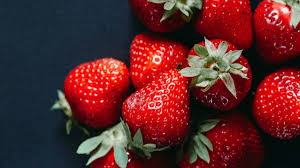
\includegraphics[width=\textwidth]{Figures/fruit1.jpeg}
    \caption{First subfigure.}
    \label{fig:first}
\end{subfigure}
\hfill
\begin{subfigure}{0.4\textwidth}
    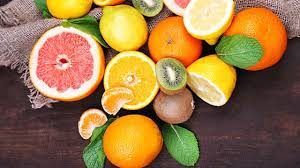
\includegraphics[width=\textwidth]{Figures/fruit2.jpeg}
    \caption{Second subfigure.}
    \label{fig:second}
\end{subfigure}
\hfill
\begin{subfigure}{0.4\textwidth}
    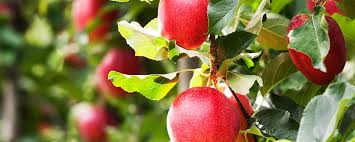
\includegraphics[width=\textwidth]{Figures/fruit3.jpeg}
    \caption{Third subfigure.}
    \label{fig:third}
\end{subfigure}
        
\caption{Creating subfigures.}
\label{fig:figures}
\end{figure}

\section{Section 2 Heading}

Contents

\subsection{Subsection Heading}

Contents
	
	\section{Summary and Gaps Identified}
	\paragraph\ 
	This is the most important section of Chapter 2. This subsection has two parts (i) summary 	and (ii) gaps identified. Summary can be a tabular form mentioning the advantages/disadvantages associated with each title. The gaps identified can be a numbered list of around four or five points mentioning what is lacking in the current state of art.
	
	Chapter conclusion goes here.